% !TEX TS-program = lualatex
%%%%%%%%%%%%%%%%%% USAGE INSTRUCTIONS %%%%%%%%%%%%%%%%%%
% - Compile using LuaLaTeX and biber, unless there is a particular reason not to. Do not use the older LaTex/PDFLaTeX or BibTeX. (The fonts won't work correctly.)
% - Expect to get 2 warnings when working correctly, one on xcolor and hyperref, and one on ExtSizes saying is better to use a class. These can be ignored.
% - Font and the report 'year' must be specified when all \documentclass or the template won't work correctly. (There's no error checking/default cases!)
% - For best performance save images/graphics as PDF files, not as png/jpg/eps. This makes no difference to how images are inserted using \includegraphics.
% - As many further packages as wanted can be loaded. Below are just an example set. Note that template itself loads a number of packages, including hyperref.
% - References are handed using biblatex.
% - Link to the presentation of dissertations policy: https://documents.manchester.ac.uk/display.aspx?DocID=2863



%%%%%%%%%%%%%%%%%% META DATA SETUP %%%%%%%%%%%%%%%%%%
% This is where the document title and author are set. Other details for the title page are set later
% Note that if/when you edit these you may need to 'Recompile from scratch' to get the changes to display in the PDF. (In Overleaf, select the down arrow to the right of the 'Recompile' button)
\begin{filecontents*}{\jobname.xmpdata}
  \Title{BEng final dissertation} 
  \Author{11006231} % should be student number rather than name to help with annoymous marking
  \Language{en-GB}
  \Copyrighted{True}
  % More meta-data fielda can be added here if wanted, see https://ctan.org/pkg/pdfx?lang=en for fields
\end{filecontents*}

\newcommand{\newtitle}{Comparing Arm Tracking Teleoperation to Conventional Joystick Control of a Laterally Mounted Robot Arm }
\newcommand{\mystudentid}{11006231}

%%%%%%%%%%%%%%%%%% DOCUMENT SETUP %%%%%%%%%%%%%%%%%%
\documentclass[12pt,beng]{uom_eee_dissertation_casson} % course can be msc or beng
% Check your course handbook for the correct font size to use. Make sure this is correct - you may get an overlength penalty if not! Is currently 12 for BEng, and 11 for MSc. The template doesn't change this automatically for you


%%%%%%%%%%%%%%%%%% PACKAGES AND COMMANDS %%%%%%%%%%%%%%%%%%

% Packages
\usepackage{graphicx}              % for adding graphics files
  \graphicspath{ {./images/} }
\usepackage{amsmath}               % assumes amsmath package installed
  \allowdisplaybreaks[1]           % allow eqnarrays to break across pages
\usepackage{amssymb}               % assumes amsmath package installed 
\usepackage{url}                   % format hyperlinks correctly
\usepackage{rotating}              % allow portrait figures and tables
\usepackage{multirow}              % allows merging of rows in tables
\usepackage{lscape}                % allows pages to be typeset in landscape mode
\usepackage{tabularx}              % allows fixed width tables
\usepackage{verbatim}              % enhanced version of built-in verbatim environment
\usepackage{footnote}              % allows more control over footnote environments
\usepackage{float}                 % allows H option on floats to force here placement
\usepackage{booktabs}              % improve table line spacing
\usepackage{lipsum}                % for adding dummy text here
\usepackage[base]{babel}           % required for lisum package
\usepackage{subcaption}            % for multiple sub-figures in a single float
\usepackage{siunitx}               % add SI units
% Add your packages here


% Custom commands
\newcommand{\degree}{\ensuremath{^\circ}}
\newcommand{\sus}[1]{$^{\mbox{\scriptsize #1}}$} % superscript in text (e.g. 1st)
\newcommand{\sub}[1]{$_{\mbox{\scriptsize #1}}$} % subscript in text
\newcommand{\otoprule}{\midrule[\heavyrulewidth]}
\newcolumntype{Z}{>{\centering\arraybackslash}X}  % tabularx centered columns 
% Add your custom commands here



%%%%%%%%%%%%%%%%%% REFERENCES SETUP %%%%%%%%%%%%%%%%%%

% Setup your references here. Change the reference style here if wanted
\usepackage[style=ieee,backend=biber,backref=true,hyperref=auto,maxbibnames=3,minbibnames=1]{biblatex}
% Note backref=true adds a page number (and hyperlink) to each reference so you can easily go back from the references to the main document. You may prefer backref=false if you need to stick strictly to a given reference style


% Fixes which can't be applied in the .cls file
\DefineBibliographyStrings{english}{backrefpage = {cited on p\adddot},  backrefpages = {cited on pp\adddot}}
%  \renewcommand*{\bibfont}{\large}


% Add more .bib files here if wanted
\addbibresource{references.bib}



%%%%%%%%%%%%%%%%%% AUTOMATIC WORD COUNT SETUP %%%%%%%%%%%%%%%%%%
% Automatically counts the words present and makes a \mywordcount variable. This is used later to automatically add the word count (which can be overridden if wanted)
% See https://www.overleaf.com/learn/how-to/Is_there_a_way_to_run_a_word_count_that_doesn%27t_include_LaTeX_commands%3F for info on what words are counted and how to control this. Any changes to what's counted need to be made in uom_thesis_casson.cls, in the \newcommand{\quickwordcount} command. The default doesn't count words in headings, captions, or references and so you may get slightly different numbers if use a different word count tool
% This can be a bit fragile. If it doesn't work, there's an option later on to just type in a numer
% \quickwordcount{\currfilebase} % run word count. This just counts the words. Is displayed with the \wordcount command later



%%%%%%%%%%%%%%%%%% START DOCUMENT %%%%%%%%%%%%%%%%%%

% Don't edit these lines, title and author are automatically taken from the document meta-data defined above
\begin{document}
\makeatletter
\title{\newtitle}
\studentid{\mystudentid}
\makeatother

% Set the below yourself
\course{Electronic Engineering}  % "Master of Science in" or "Bachelor of Engineering in "
                                                   % is added automatically
                                                   % Our BEng courses are: Electrical and Electronic Engineering, Electrical Engineering, and Mechatronic Engineering
                                                   % Our MSc courses are: Advanced Control and Systems Engineering, Advanced Control and Systems Engineering with Extended Research, Communications and Signal Processing, Communications and Signal Processing with Extended Research, Electrical Power Systems Engineering, Advanced Electrical Power Systems Engineering, Renewable Energy and Clean Technology, Renewable Energy and Clean Technology with Extended Research, Robotics, Robotics with Extended Research
\faculty{Science and Engineering}                  % "Faculty of" is added automatically
\school{School of Engineering} % "School of" not added automatically (as if in AMBS, School comes at the end rather than the start), so enter full name of School here
\submitdate{2025}                                  % regulations ask only for the year, not month
\wordcount{1234}		                   % use \wordcount{} to set the count. Can just type in a number (e.g. \wordcount{1000}	if don't want to use the automatic count.) This is automatically displayed after the table of contents. 
\maketitle



%%%%%%%%%%%%%%%%%% LISTS OF CONTENT %%%%%%%%%%%%%%%%%%
\uomtoc
% other lists are not required, but can include \uomlof and \uomlot if really want to


%%%%%%%%%%%%%%%%%% ABSTRACT %%%%%%%%%%%%%%%%%%
\begin{abstract} % put abstract here.
  Abstract goes here.
\end{abstract}%
\clearpage



%%%%%%%%%%%%%%%%%% DECLARATIONS %%%%%%%%%%%%%%%%%%
\begin{uomoriginality}
  \uomoriginalitydeclaration 
  % If the standard originality decalaration is sufficient, saying no portion of the work has been submitted in support of an application for another degree or qualification, the above command will automatically add the required text and nothing else is needed in this section.
  % If the standard statment isn't sufficient, then comment out the \uomoriginalitydeclaration command and type in your own text here explaining the authorship of any re-used portions. 
\end{uomoriginality}
\uomcopyrightstatement



%%%%%%%%%%%%%%%%%% ACKNOWLEDGEMENTS %%%%%%%%%%%%%%%%%%
\begin{uomacknowledgements}
Acknowledgments go here.
\end{uomacknowledgements}



%%%%%%%%%%%%%%%%%% Start content %%%%%%%%%%%%%%%%%%
\uomstartmainbody % Don't delete. used to flag to the hyperlinks in the PDF that the main content is  starting



%%%%%%%%%%%%%%%%%% INTRODUCTION %%%%%%%%%%%%%%%%%%
\section{Introduction} % can use \input{} or \include{} for each section to draw content from other files rather than having everything in one big file
  
  The goal of this project is to create a system for controlling and teleoperating a robot arm with a human arm. 
  In order to maintain simplicity in the project scope, the robot arm is assumed to be shoulder-mounted and has the seven degrees of freedom (DoF) \cite{ref:arm_dofs}, matching that of a healthy human arm.
  An example of the humanoid robot arm (the YuMi robot) is shown in figure \ref{fig:yumi}.

  \begin{figure}[h!]
      \centering
      \includegraphics[scale=0.3]{images/yumi_two_arms.png}
      \caption{YuMi Robot Arm To Be Used In Experiment}
      \label{fig:yumi}
    \end{figure}

  \subsection{Background and motivation}
  The motivation for this project comes from articles within the books: \citetitle{ref:Zhou_Yang_Wang_Dong_2025} \cite{ref:Zhou_Yang_Wang_Dong_2025} and \citetitle{ref:Lyu_Yang_Yang_2025} \cite{ref:Lyu_Yang_Yang_2025}.
  Both of these articles use an inertial measurment unit (IMU) to gather data, but only maps the wrist position to the robot's end effector.

  Redundancy in the degrees of freedom of the arm means that a valid end effector position can have multiple positions of the previous links \cite{ref:nullspace}.
  Therefore this ambiguity could lead to collisions with obstacles in the environment, and lack of safety for people within the envelope of the robot arm. 
  
  Some specific use cases will require absolute control of every link of the robot arm - for example underwater sample collection.
  Whilst \citeauthor{ref:Jin_Ji_Yan_2023} describes a potential autonomous solution \cite{ref:Jin_Ji_Yan_2023}, this method is comparatively slow to the prospect of remote teleoperation.
  Consequently, the complexity increase for the case where nothing is stationary, a more realistic use case, would mean that this method would be inefficient compared to the intuition of a trained operator. 
  
  Additionally, \citeauthor{ref:vranalysis} shows that for tasks involving teleoperation of a robot for pick and place tasks, virtual reality style mapping of head movements with arm to end effector mapping is more efficient and less error prone than a typical joystick \cite{ref:vranalysis}.
  Hence, exploration of the performance characteristics between conventional control methods and arm mapped teleoperation is undertaken.

  \subsection{Aims and objectives}
  The overall aim is to compare the performance of a system for mapping the joint angles of a human arm to a shoulder-mounted robot arm to conventional control methods. 
  This will include:

  \begin{itemize}
    \item Identifying and comparing existing technologies, including IMU based solutions discussed earlier, attitude and heading reference systems \cite{ref:Mazomenos_Biswas_Cranny_Rajan_Maharatna_Achner_Klemke_Jobges_Ortmann_Langendorfer_2016}, computer vision based systems \cite{ref:Phuong_Cong_2024}, and flex sensor based systems \cite{ref:Nalam_Manivannan_2014}.
    \item Developing a version of the tracking system suitable for controlling a simulation of the YuMi robot arm.
    \item Devising experiments appropriate to comparing conventional methods of control to arm tracking teleoperation methods.
    \item Analysing the difference, if any, in performance between either method of control in a variety of environments.
  \end{itemize}

%%%%%%%%%%%%%%%%%% LITERATURE REVIEW %%%%%%%%%%%%%%%%%%
\section{Examination of existing human to robot arm teleoperation methods}

  This section explores which arm tracking methods are the most suitable for this project.
  Quantitative and qualitative data from secondary research is used to create a justified specification for the final solution.
  Finally, a Pugh matrix will be applied to fairly score and select an appropriate method to further develop.

\label{sec:litrev}

  \subsection{Why choose teleoperation over conventional input methods}
    The measurement of human arm joint angles has been an interest of academia for several decades: with one of the first examples being demonstrated by \citeauthor{ref:videobasedumanmotioncapture}. 
    In industrial settings, full body tracking has primarily been used in the film industry to accurately measure an actor's performance \cite{ref:mocapwhy} and map them onto computer generated characters \cite{ref:whatmocap}.
    
    This approach could also be applied to the control of robotics: have a skilled operator remotely control industrial robots where traditional control methods (e.g. joysticks) are unsuitable.
    Research has shown that this approach could lead to \num{1.8} times faster task completion time and with a quarter of the errors (\(1.54 \% \) compared to \(8.65 \% \)) in the best cases  \cite{ref:vranalysis}. 

    Another way to increase the performance of a task with teleoperation is mapping the head movements of an operator to the camera of the robot performing the task \cite{ref:teleopanalysis}.
    However, this study was based primarily on the control of wheeled robots; manual joystick controls exceeded the performance of teleoperation in this specific task.
    
    These two cases suggests that whether teleoperation is more effective than traditional joysticks is strongly dependent on the task.
    Overall, in the case of robot arm control, there is potential for performance increases via human arm teleoperation \cite{ref:Zhou_Yang_Wang_Dong_2025}, strengthening the justification for this project.

  \subsection{Requirements of a suitable tracking system}
    In order to compare the final system to existing systems and research, desired characteristics must be identified.
    
    \begin{description}
      \item[Accuracy requirements] - Be able to measure joint rotations with a minimum resolution of \(3 \degree\). 
      
      Experienced surgeons have been measured to have \(5 \degree\) of vertical movement range on all joints when asked to hold their hand on a target, and close to \(3 \degree\) range for horizontal movement \cite{ref:movementrange}.
      Therefore any measurement lower than this resolution can be characterised as 'noise' from human inaccuracy, and can be smoothed out.
      \item[Latency requirements] - Have a maximum system latency of \(300 \text{ ms}\). 
      
      Teleoperation task performance generally degrades around the two key figures of \(600 \text{ ms}\) and \(1500 \text{ ms}\) \cite{ref:teleoplatency}.
      Thus, the Nyquist criterion equivalent of this threshold is used as a well informed estimate of how much latency can be present in the system, leaving a final requirement of \(300 \text{ ms}\).
      
      \item[Resource requirements] -  The budget for this project is \(£180\), and \(30\) unit credits worth of time, equating to \(240\) hours of time commitment.
      
      Both of these factors will mean that the final solution favours simpler, more complete solutions. 
      Anything novel is a potential failure point that could mean the project does not complete.  
    \end{description}

  \subsection{Survey of existing tracking technologies}
    In order to fully evaluate the myriad of arm tracking methods available, a Pugh Matrix has been created (see \autoref{tab:pugh_matrix_detailed}) to evaluate and compare several factors between each method.
    Each method will score \(1 - 5\) in each category, with a brief comment justifying the score in each column.
    
    Below are the decision factors of the Pugh Matrix and a brief description of how they are scored: \begin {description}
      \item \textbf{Complexity} - This is calculated based on a well reasoned estimate of the total time to build the system. Each multiple of \(48\) hours reduces the score by \(1\), e.g. \(0 - 48\text{ hours}\) would score \(5\), \(49 - 96\text{ hours}\) would score \(4\).
      \item \textbf{Cheapness} - This is calculated based on a well reasoned estimate of the total cost of building the system. Each multiple of \(£36\) reduces the score by \(1\), e.g. \(\text{£}0 - \text{£}36\) would score \(5\), \(\text{£}37 - \text{£}72\) would score \(4\).
      \item \textbf{Accuracy} - This is calculated from available research on the accuracy of this method. Each multiple of \(5 \degree\) above \(5 \degree\) reduces the score by \(1\), e.g. an absolute accuracy of \(6 - 10 \degree\) would score \(4\), \(11 - 15 \degree\) would score \(3\).
      \item \textbf{Latency} - This is calculated from available research on the time it takes to obtain a single measurement of all 7 joint angles from this method. Each multiple of \(100 \text{ ms}\) above \(300 \text{ ms}\) reduces the score by \(1\), e.g. a latency of \(301 \text{ ms} - 400 \text{ ms}\) would score \(4\).
    \end{description}

    Analysis of existing methods shows that the two computer vision approaches score similarly in terms of viability, therefore further analysis will be required to confirm the viability of each method.
    These will be performed in the form of accuracy and latency experiments.
    This has the advantage of being able to examine more factors than existing literature - of particular interest is the accuracy of measuring multiple joints angles simultaneously.
    
    In particular, the potential accuracy advantage of the marker tracking method makes it more appealing, though this is offset by the stupendous cost of conventional Vicon camera systems.
    However, open source software along with ArUco markers could be used to offset this cost - which is worth exploring before committing to any substantial development.
    For example, \citeauthor{ref:arucomarkers} describes using ArUco markers along with standard home cameras to perform specialised kinematic analysis \cite{ref:arucomarkers}.
    
    \begin{table}[h]
      \centering
      \caption{Pugh Matrix with detailed scoring justifications}
      \small
      \begin{tabular}{>{\raggedright\arraybackslash}p{2.5cm}|>{\centering\arraybackslash}p{1.8cm}|>{\centering\arraybackslash}p{1.8cm}|>{\centering\arraybackslash}p{1.8cm}|>{\centering\arraybackslash}p{1.8cm}|c}
      \toprule
      \textbf{Method} & \textbf{Complexity \(1-5\)} & \textbf{Cheapness \(1-5\)} & \textbf{Accuracy \(1-5\)} & \textbf{Latency (\(1-5\))} & \textbf{Total} \\
      \midrule
      Pose estimation via computer vision & \(5\) & \(5\) & \(3\) & \(5\) & \(18\) \\
       & Existing solutions reduce complexity \(30 - 40\text{ hours}\) & £\(30\) USB Camera & \(10\degree-15\degree\) \cite{ref:cverror} & \(\le 100 \text{ ms}\) \cite{ref:cvlatency} & \\
      \midrule
      Marker tracking via computer vision & \(5\) & \(3\) & \(5\) & \(5\) & \(18\) \\
       & Very complex, though can be simplified through FOSS & £180+ for Vicon, cheaper solutions exist & <5° error & 100-200ms & \\
       \midrule
      IMU-based & \(3\) & \(4\) & \(3\) & \(5\) & \(15\) \\
       & \(100\text{ hours}\) including PCB design + drift correction & £\(50-\text{£}60\) & \(2.8 \degree\) \cite{ref:imuerror} & <1 ms \cite{ref:imudatasheet} & \\
      \midrule
      Flex Sensors & 2 & 4 & 4 & 5 & 15 \\
       & \(150 \text{ hours}\) & £40-60 & \(10\degree\) \cite{ref:bendaccuracy} & \(\le 100 \text{ ms}\) & \\
      \bottomrule
      \end{tabular}
      \label{tab:pugh_matrix_detailed}
    \end{table}

%%%%%%%%%%%%%%%%%% METHODS %%%%%%%%%%%%%%%%%%
% \pagebreak
\section{Comparing two viable computer vision based methods of robot arm teleoperation} \label{sec:methods}

The criteria selected both ArUco marker tracking and pose estimation as equally viable methods of human arm tracking. 
This section aims to develop a minimum viable product (MVP) version of both methods to be used to quantify which approach is more suitable for the final solution.

\label{sec:methods}

  \subsection{Comparison of both computer vision methods}
    In order to evaluate the accuracy of both computer vision methods, a simple experiment was set up to measure the absolute accuracy on the joint angles that can be measured.
    A goniometer is attached to the wall at \(90 \degree\), with two end positions marked at \(90 \degree\) and \(180 \degree\).
    The subject will move their arm repeatedly between these markers, and the recording is captured by a camera as described in \autoref{fig:datacollection}.

    \begin{figure}[h!]
      \centering
      \begin{subfigure}[b]{0.4\linewidth}
        \includegraphics[width=\linewidth]{images/experiment2d.png}
        \caption{A diagram of the experimental setup.}
      \end{subfigure}
      \begin{subfigure}[b]{0.4\linewidth}
        \includegraphics[width=\linewidth]{images/experimentdataimg.png}
        \caption{Example data capture}
      \end{subfigure}
      \caption{The experimental setup, showing data capture.}
      \label{fig:datacollection}
    \end{figure}

    The subject will then flex and extend their elbow between the two endpoints. 
    In order to obtain a sufficient amount of data, \(5\) videos are recorded, each showing \(10\) flexion and extensions.

    This creates enough samples to perform ANOVA between each video, to maintain experimental integrity.
    In order to measure error, the graph of elbow flexion angles is extended towards the \(90 \degree\) and \(180 \degree\) endpoints.
    This secondary graph is then subtracted from the first graph to obtain the error value, from which we can calculate the root mean square error, and is shown in \autoref{fig:elbow_flex_example}.

    \begin{figure}[!htb]
      \centering
      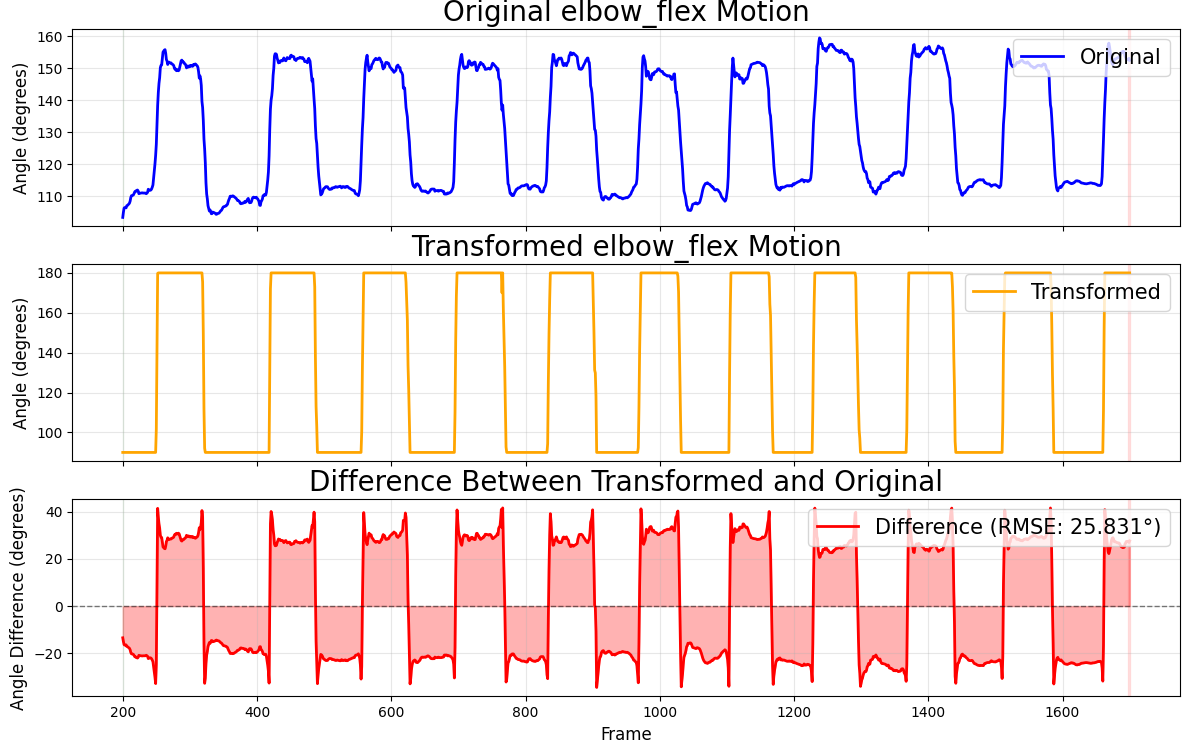
\includegraphics[width=0.8\linewidth]{images/elbow_flex_graph_v2.png}
      \caption{Showing how RMSE is calculated from elbow flexion data.}
      \label{fig:elbow_flex_example}
    \end{figure}

    Upon analysis of the RMSE, it was found that this value was \(25.83 \degree\).
    which was greater than the literature value of \(10.37 \degree\) \cite{ref:cverror}. 
    Frame by frame analysis of the video showed that this descrepancy was not attributable to human error - the arm was clearly flexing and extending to the correct endpoints.
    
    Plotting the inferred joint positions frame by frame revealed the culprit - perspective!
    The machine learning model used for joint position extraction is finding extra movement in the depth axis of the video, and attributing it to roll in the elbow axis, instead of flexion.
    This is clearly shown in \autoref{fig:phantom_flex}.

    To analyse the performance of joint angle tracking in the three dimensional case, a simple movement path is created. 
    A 7 DoF manipulator is created from relevant DH parameters (specifics found in appendix \autoref{tab:dh_parameters})
    These movements are then fed through a forward kinematics processing program to obtain a visualisation of this movement path, and this movement is recreated by the subject.
    
    \begin{figure}[H]
      \centering
      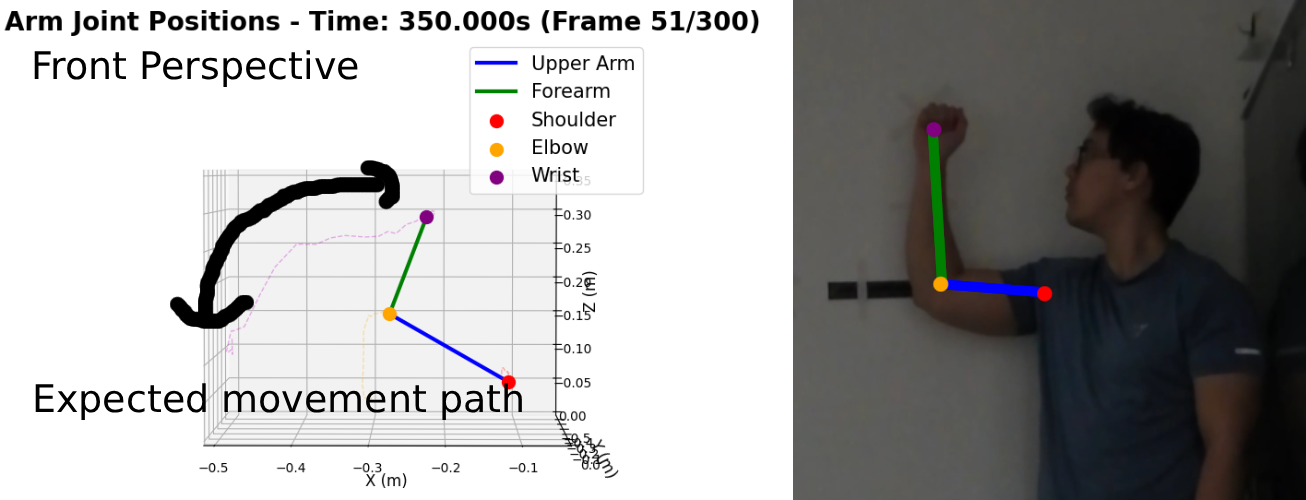
\includegraphics[width=0.7\linewidth]{images/frontperspective.png}
      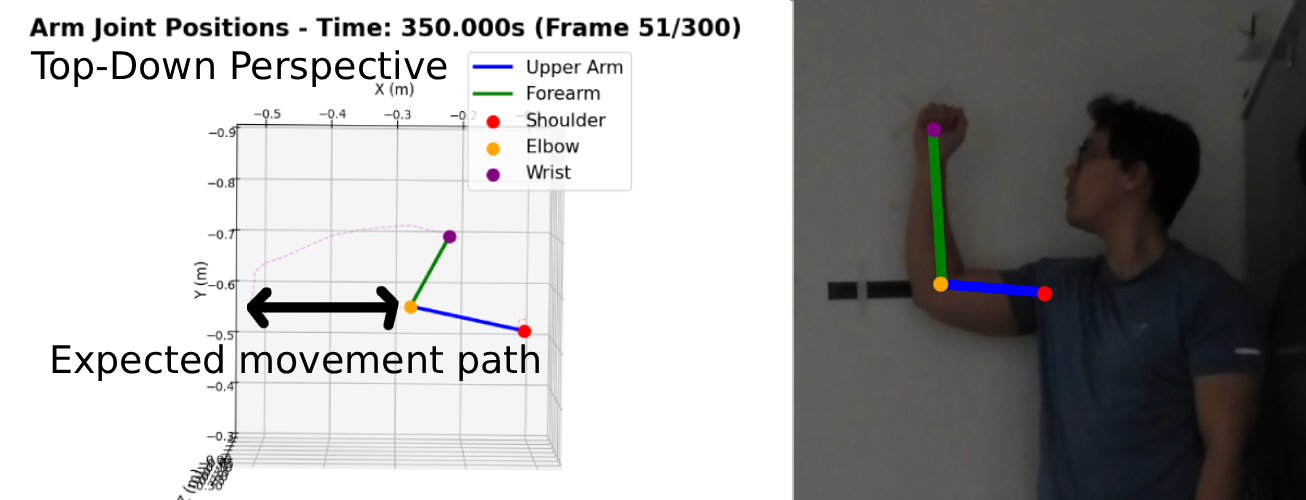
\includegraphics[width=0.7\linewidth]{images/topdown_perspective.png}
      \caption{Front and top view of inferred \(3\)D joint positions.}
      \label{fig:phantom_flex}
    \end{figure}

    This path is shown in \ref{fig:threed_motion}.
    This movement has been selected to be easily recreated, whilst showing movement in three different joint angles simultaneously. 
    The same data processing for the two dimensional elbow flex case is used to obtain RMSE of three different joint angle movements.

    \begin{figure}[!htb]
        \centering
        \includegraphics[scale=0.5]{images/combination.png}
        \caption{3D Joint Motion Path}
        \label{fig:threed_motion}
    \end{figure}

  \subsection{Results of joint angle tracking methods}
    Table \ref{tab:rmse_comparison} shows the compiled RMSE errors for tracking each joint in both the two dimension elbow flexing case and the three dimension movement path.

    \begin{table}[h]
      \label{tab:rmse_comparison}
      \centering
      \small
      \begin{tabular}{>{\raggedright\arraybackslash}p{3cm}|>{\centering\arraybackslash}p{2.5cm}|>{\centering\arraybackslash}p{2.5cm}|>{\centering\arraybackslash}p{2.5cm}|>{\centering\arraybackslash}p{2.5cm}}
      \toprule
      \textbf{Method} & \textbf{RMSE Error Elbow Flexion 2D (\(\degree\))} & \textbf{RMSE Error Elbow Flexion 3D (\(\degree\))} & \textbf{RMSE Error Shoulder Flexion (\(\degree\))} & \textbf{RMSE Error Shoulder Abduction (\(\degree\))} \\
      \midrule
      Pose estimation & 25.83 & 7.19 & 6.89 & 11.68 \\
      \midrule
      Marker Tracking & N/A & N/A & N/A & N/A \\
      \bottomrule
      \end{tabular}
      \caption{RMSE error of either tracking method}
    \end{table}

    Whilst the two dimensional RMSE error is larger than the literature suggests, the three dimensional joint error shows better accuracy than expected.
    Apart from the shoulder adduction/abduction measurements, each joint being tracked is almost in the same order of magnitude of the \(3 \degree\) requirements of the project.
      
    Despite various attempts, ArUco marker tracking seemed to be too unstable in this specific application. 
    Both 2D paper markers and 3D printed markers were used, though the glossy surface finish of either meant that tracking was unreliable at close distances and impossible at moderate distances.
    This was obtained from an experiment wherein a marker is held up to the camera and rotated around various axes, measuring the captured rotation.
    
    \autoref{fig:arucomarkerresults} shows a plot of the measured roll angle, and shows the gaps in which no measurement was made.
    Clearly this level of unreliability is unsuitable for the final tracking task, and therefore no further testing will be required.

    \begin{figure}[h!]
      \centering
      \includegraphics[width=\linewidth]{images/measuredrollangle.png}
      \caption{Measured vs Expected graph of pitch of ArUco marker}
      \label{fig:arucomarkerresults}
    \end{figure}

    An interesting aspect that was encountered when performing the accuracy characterisation experiments with pose estimation is shown in \autoref{fig:weezered}, and points to a downside not immediately apparent.
    The program uses machine learning to create an estimation of joint locations in an image and was ostensibly trained on a large corpus of human images.
    Hence, there was trouble distinguishing between real humans and pictures of humans being worn on the subject's clothing - a downside in the favour of the marker tracking method.

    \begin{figure}[h!]
      \centering
      \includegraphics[scale=0.8]{images/weezered.png}
      \caption{Pose estimation software mistaking a picture of humans printed on the clothing for an actual person.}
      \label{fig:weezered}
    \end{figure}

  \subsection{Final Tracking Method}

  Results show that the pose estimation is roughly able to achieve the \(5 \degree\) measurements required for the project.
  Moreover, the mediapipe model used to power this is optimised for real time measurement; using a \(30 \text{ fps}\) camera, each measurement takes \(33 \text{ ms}\), well below the required \(300 \text{ ms}\).
  Hence, the comparison between conventional joystick control and human arm tracking teleoperation will use the pose estimation approach for comparison.

%%%%%%%%%%%%%%%%%% RESULTS %%%%%%%%%%%%%%%%%%
% \pagebreak
\section{Experiments to characterise the difference in performance of arm tracking vs conventional control methods} \label{sec:results}
\label{sec:experiments}

  \subsection{Description of experiment to compare conventional vs human arm tracking}
    In order to compare fairly the two methods of control, three scenarios will be examined:

    \begin{description}
      \item[\autoref{sec:scen1}] - Position matching task similar to \citeauthor{ref:movementrange} \cite{ref:movementrange}. 
      A random location within the envelope of the arm is selected and the operator must control the arm to this location as fast as possible.
      \item[\autoref{sec:scen2}] - Pick and place task. 
      An object and target location spawns within the envelope of the arm, and the operator must manipulate the object to the target.
      \item[\autoref{sec:scen3}] - Obstacle laden pick and place task. 
      Similar to pick and place task, but with tracking of obstacle collisions.
    \end{description}

    The operator must stand further away from the screen to be in frame of the camera for the pose estimation method.
    To negate the perception advantages this would incur for the controller tasks, the controller method will be performed sitting this same distance away. 

    Scenarios \(2\) and \(3\) consist of four different phases shown in \autoref{fig:pickandplacephases}
    The object is considered 'held' as long as YuMi's grippers are within a certain distance threshold, and transition from an open state to a closed state.
    This prevents the experiment from being limited by the design and simulation of a suitable end effector - though this may act as an interesting extension for future research.

    To measure the performance of the position matching task, the distance covered is divided by the time taken to find the normalised speed measurement.
    To measure the performance of the pick and place task, the cumulative time spent in each phase is measured, along with the overall time to complete the task.
    Likewise, to ensure fairness between each method in both pick and place tasks, seeded randomness will be used to ensure that both methods get the same trial spawn position.

    \begin{figure}[h!]
      \centering
      \begin{subfigure}{0.3\linewidth}
          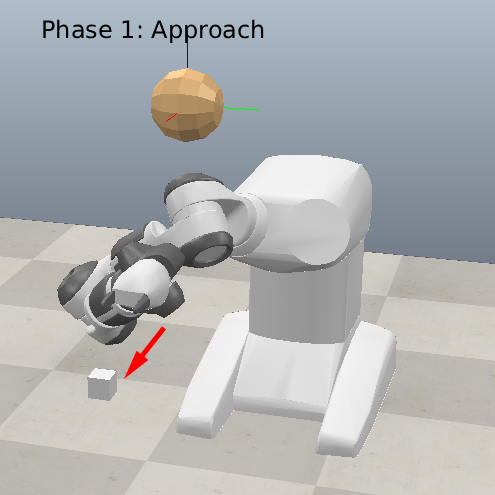
\includegraphics[width=\linewidth]{images/approach.png}
          \label{fig:image1}
      \end{subfigure} 
      \hspace{0.75em}
      \begin{subfigure}{0.3\linewidth}
          \includegraphics[width=\linewidth]{images/grip.png}
          \label{fig:image2}
      \end{subfigure}

      \begin{subfigure}{0.3\linewidth}
          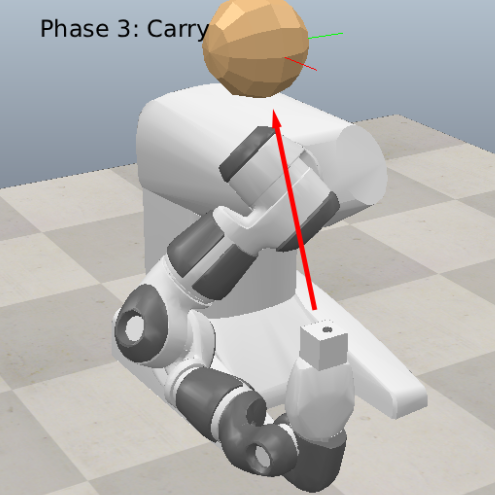
\includegraphics[width=\linewidth]{images/carry.png}
          \label{fig:image3}
      \end{subfigure}
      \hspace{0.75em}
      \begin{subfigure}{0.3\linewidth}
          \includegraphics[width=\linewidth]{images/place.png}
          \label{fig:image4}
      \end{subfigure}

      \caption{Phases of the pick and place scenario}
      \label{fig:pickandplacephases}
    \end{figure}
  
  \subsection{Scenario 1: Random position matching task}
  \label{sec:scen1}
  \(100\) samples were taken, with \(10\) runs of \(10\) experiments. 
  Analysis of variance (ANOVA) shows no significant deviation between each run (see appendix \textbf{TODO figure this out}).
  The controller method was roughly \(42 \%\) faster than the pose estimation algorithm, although with a lower standard deviation of 0.043 compared to 0.053.
  
  The speed difference is likely attributable to the operator's familiarity of using controllers in video games, boasting over \(10\) years of meaningful experience in this field.
  Notably, the difference in standard deviation could imply that pose estimation is stronger for tasks that require consistency, rather than outright speed.

  \begin{figure}[h!]
    \centering
    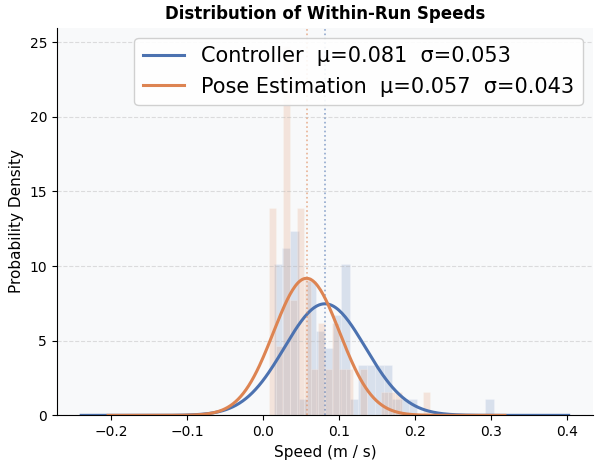
\includegraphics[width=\linewidth]{images/reach_experiment_results.png}
    \caption{Standard distribution plot of the results of either experiment}
    \label{fig:experiment1res}
  \end{figure}
    
	\subsection{Scenario 2: Simple environment pick and place task}
  \label{sec:scen2}

  The pose estimation algorithm shows \(60.3 \%\) reduction in time over the controller control in this task, with the noticeable difference being in the proportion of time spent in the 'approach' phase (see \autoref{fig:experiment2res})
  The controller method requires the operator to orient the gripper over the object, and doing this in certain arm positions can lead to singularities in the inverse kinematics solver, hence the longer time.
  
  These singularities can be seen in a joint angle over time plot of one of the experiments in \autoref{fig:singularities}.
  The advantage of the pose estimation method is that the human arm of the operator acts as a safety net for unreachable positions.

  \begin{figure}[h!]
    \centering
    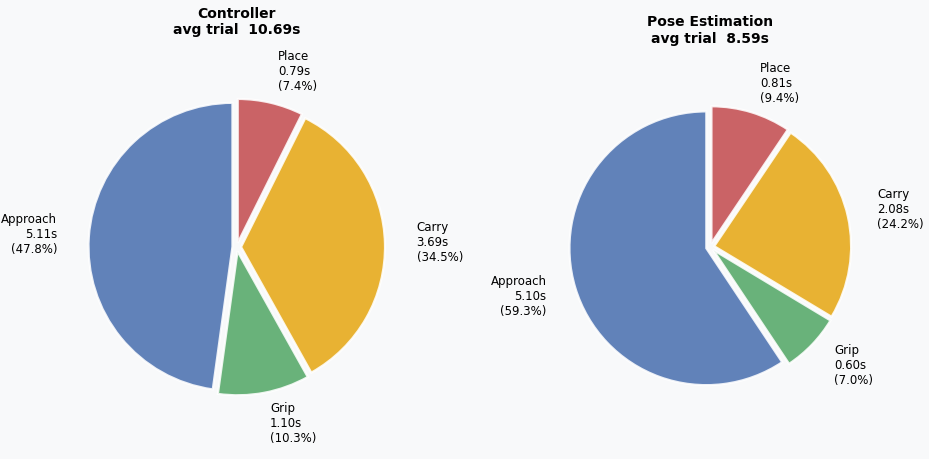
\includegraphics[width=\linewidth]{images/transport_results.png}
    \caption{Standard distribution plot of the results of either experiment}
    \label{fig:experiment2res}
  \end{figure}


  \begin{figure}[h!]
    \centering
    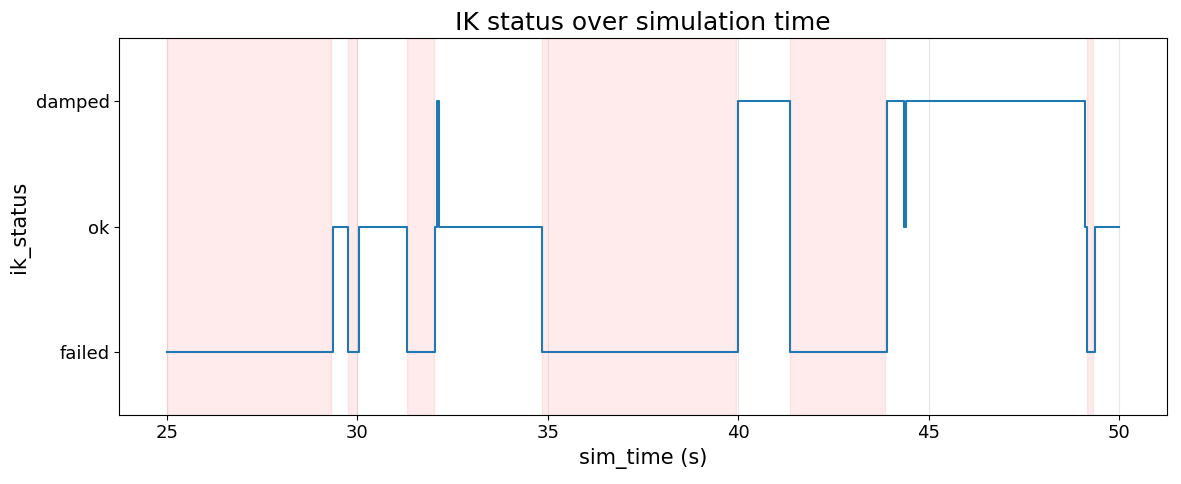
\includegraphics[width=\linewidth]{images/jointangletime.png}
    \caption{Joint angle over time plot of the robot arm during a controller experiment }
    \label{fig:singularities}
  \end{figure}
  
        
    
	\subsection{Scenario 3: Obstacle-rich environment pick and place task}
  \label{sec:scen3}

  The pose estimation algorithm is quicker on average by \(57.2 \%\) in this task, likely for the same reasons as above - where the controller solution is running into singularities.
  Additionally, the added dexterity shown led to \(3.46\) fewer collisions (\(4.14\) vs \(7.60\)) on average compared to the controller solution.

  The fewer collisions may be due to more control that the operator has over the entire arm, as more data can be transmitted from the operator to the robot, in a way that is intuitive.
  Likewise, the smooth control of the pose estimation algorithm may make it more predictable compared to the IK approach of the controller solution - where it may be jumping over singularity positions unpredictably.

  The proportion of time spent in the approach phase increased by \(9 \%\) for the pose estimation solution, and decreased by \(66.8 \%\) for the controller solution.
  Interestingly, the controller solution becomes more balanced in the time spent in each movement phase, whereas the pose estimation solution becomes front loaded.

  There is also a noticeable difference in the average trial time between scenario 3 and scenario 2, likely attributable to the operator becoming more skilled and experience with each control method and experiment.

  \begin{figure}[h!]
    \centering
    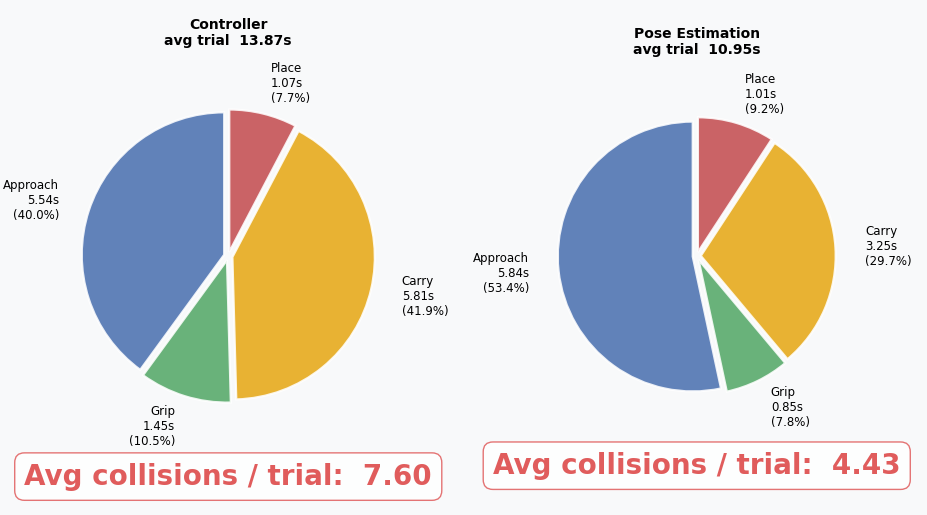
\includegraphics[width=\linewidth]{images/obstacle_results.png}
    \caption{Standard distribution plot of the results of either experiment}
    \label{fig:experiment3res}
  \end{figure}



%%%%%%%%%%%%%%%%%% CONCLUSIONS %%%%%%%%%%%%%%%%%%
\section{Conclusions and future work} % edit subsection heading as appropriate
\label{sec:conc}
  \subsection{Conclusions}
	

	\subsection{Future work}



%%%%%%%%%%%%%%%%%% REFERENCES %%%%%%%%%%%%%%%%%%
%\clearpage % uncomment to start on a new page if wanted
\printbibliography[title={References},heading=bibintoc] % a single list of references for the whole thesis



%%%%%%%%%%%%%%%%%% APPENDICES %%%%%%%%%%%%%%%%%%
\begin{uomappendix} 
    \section{Project outline}
    Project outline as submitted at the start of the project is a required appendix. Put here. 
    
    \section{Risk assessment}
    Risk assessment is a required appendix. Put here.\

    \section{DH Parameters}
    The DH parameters used for the arm are as follows:

    \begin{table}[h]
      \centering
      \small
      \begin{tabular}{>{\centering\arraybackslash}p{1.2cm}|>{\raggedright\arraybackslash}p{3.5cm}|>{\centering\arraybackslash}p{1.5cm}|>{\centering\arraybackslash}p{1.5cm}|>{\centering\arraybackslash}p{1.5cm}|>{\centering\arraybackslash}p{1.5cm}}
      \toprule
      \textbf{Joint} & \textbf{Description} & \(\boldsymbol{\theta_i}\) & \(\boldsymbol{\alpha_i}\) & \(\boldsymbol{d_i}\) & \(\boldsymbol{a_i}\) \\
      \midrule
      1 & Shoulder abduction/adduction & \(q_1\) & \(\frac{\pi}{2}\) & 0 & 0 \\
      \midrule
      2 & Shoulder flexion/extension & \(q_2\) & \(\frac{\pi}{2}\) & 0 & 0 \\
      \midrule
      3 & Shoulder rotation & \(q_3\) & \(-\frac{\pi}{2}\) & 0 & \(L_u\) \\
      \midrule
      4 & Elbow flexion/extension & \(q_4\) & \(\frac{\pi}{2}\) & 0 & 0 \\
      \midrule
      5 & Forearm rotation & \(q_5\) & \(-\frac{\pi}{2}\) & 0 & \(L_l\) \\
      \midrule
      6 & Wrist flexion/extension & \(q_6\) & \(\frac{\pi}{2}\) & 0 & 0 \\
      \midrule
      7 & Wrist radial/ulnar deviation & \(q_7\) & 0 & 0 & 0 \\
      \bottomrule
      \end{tabular}
      \caption{Denavit-Hartenberg Parameters for 7-DoF Arm (where \(L_u\) is upper arm length and \(L_l\) is lower arm length)}
      \label{tab:dh_parameters}
    \end{table}
    
    %\subsection{Other appendices as necessary}
\end{uomappendix}


%%%%%%%%%%%%%%%%%% END MATTER %%%%%%%%%%%%%%%%%%
\end{document}